\newpage
\subsection{Диагностика}
\subsubsection{Прием данных}
Прием диагностических данных в системе осуществляется через отсылку запроса на
REST API (рисунок \ref{ris:diagnostic_post_request}).

\begin{figure}[h]
\center{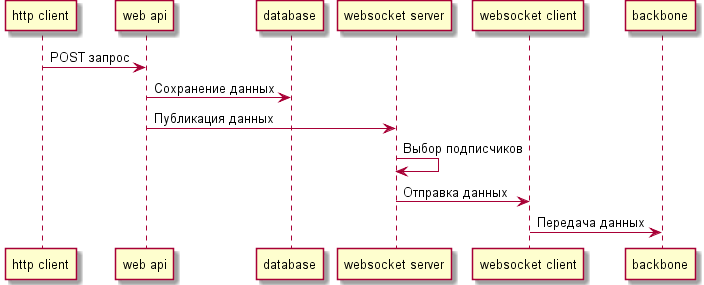
\includegraphics[width=1\linewidth]{diagnostic_post_request.eps}}
\caption{Процесс приема диагностических данных}
\label{ris:diagnostic_post_request}

% "http client" -> "web api" : POST запрос
% "web api" -> "database" : Сохранение данных
% "web api" -> "websocket server" : Публикация данных
% "websocket server" -> "websocket server" : Выбор подписчиков
% "websocket server" -> "websocket client" : Отправка данных
% "websocket client" -> "backbone" : Передача данных

\end{figure}

Запрос представляется из себя стандартный POST запрос по адресу
\url{http://localhost:3000/diagnostic/parameter} (листинг
\ref{lst:sending_diagnostic}) с указанием дополнительных параметров:
\begin{enumerate}
  \item user\_id - идентификатор пользователя в системе;
  \item parameter\_id - идентификатор мараметра;
  \item value - значение параметра.   
\end{enumerate}

\begin{lstlisting}[language=Bash,caption=Отправка диагностических данных
,label={lst:sending_diagnostic}] 
user@localhost$ curl -d "user_id=1&parameter_id=2&value=44" \
http://localhost/diagnostic/parameter
\end{lstlisting}

\subsubsection{Доступ к диагностическим данным}
Доступ к диагностическим данным предоставляется доктору. Доктор может
просматривать данные в виде графиков или таблиц. Графики формируются с помощью
класса ChartFactory в зависимости от класса параметра. ChartFactory имеет метод
build который принимет в качестве параметров:
\begin{enumerate}
  \item patient\_id - идентификатор пациента;
  \item parameter\_id - идентификатор параметра;
  \item from - начальная дата для выборки данных;
  \item to - конечная дата для выборки данных.
\end{enumerate}

Метод возвращает ассоциативный массив со структурой понятной \\ Highcharts.
После чего массив сериализуется в JSON и отдается клиенту.

\subsubsection{Публикация данных}
После поступления диагностических данных в систему, системы инициирует процесс
публикации данных (рисунок \ref{ris:diagnostic_post_request}).  Событие
указывает Websocket серверу оповестить всех заинтересованных подписчиков о том что диагностические данные обновились.

Данный механизм позволяет доктору просматривать поступающие диагностические
данные в реальном времени.

Для доступа к диагностическим данным в реальном времени используется Websocket
клиент.